\appendix

\section{Proofs}
\label{app:proofs}

Throughout, $t$ is the target, $\delta_j\in[0,u_j]$ with $u_j=\min(B,c_j-S_{tj})$ is the boost on task $j$, and a rival $i$ is beaten when the target's aggregate exceeds theirs by $\varepsilon$.

\paragraph{\Cref{prop:quantile}.}
Let the rival level be $V$, the largest rival aggregate plus $\varepsilon$. The $r$-th largest of the target's scores is at least $V$ if and only if at least $r$ of them are. The $a$ tasks already at $V$ or above count, so at least $r-a$ further tasks must be raised to $V$, which is the stated breadth. Raising a task from $S_{tj}$ to $V$ costs $d_j=V-S_{tj}$, and raising it beyond $V$, or raising a task that ends below $V$, does not help any of the $r$ positions that matter. For a set $T$ of $r-a$ tasks the least depth is $\sum_{j\in T}d_j$, minimised by the $r-a$ smallest shortfalls (exchange argument: swapping a chosen task for an unchosen one with smaller shortfall lowers the sum). The plan is feasible under $B$ and the ceilings if and only if each chosen $d_j\le u_j$, and the best choice is feasible if and only if the $(r-a)$-th smallest value of the shortfalls among tasks with $d_j\le u_j$ exists, which for tasks with equal ceilings is the condition on the $(r-a)$-th smallest shortfall stated in the proposition. The minimum is $r=m$ and the median is $r=\lceil m/2\rceil$.

\paragraph{\Cref{prop:mean}.}
With weights $w_j>0$ the target's aggregate is $A_t+\sum_jw_j\delta_j$ and first place requires $\sum_jw_j\delta_j\ge G$ (strictly, with the margin $\varepsilon$ included in $G$). The set of feasible $\delta$ is the knapsack cover $\{0\le\delta_j\le u_j,\sum_jw_j\delta_j\ge G\}$ and is non-empty if and only if $\sum_jw_ju_j\ge G$. With a linear cost $\sum_j\kappa_j\delta_j$ it is a fractional covering problem, solved by filling tasks in decreasing order of $w_j/\kappa_j$ until $G$ is covered. For the raw mean in points $w_j=1/m$ and $\kappa_j=1$, so every unit of boost buys the same $1/m$ of aggregate and the depth is $mG$ however the boost is spread. The least number of tasks that covers $G$ is the least $k$ with $\sum$ of the $k$ largest $w_ju_j$ at least $G$, because with unit cost per task it is best to take the largest headrooms. Under a convex cost the optimum equalises marginal cost per unit of aggregate across tasks that are not at their cap (water-filling).

\paragraph{\Cref{prop:rank}.}
Let the target's win count against rival $i$ on task $j$ be $1[S_{tj}>S_{ij}]+\tfrac12 1[S_{tj}=S_{ij}]$; mean rank is the sum over rivals and tasks of this quantity, divided by $m(N-1)$, and ties counted as half give the mean win rate. As a function of $\delta_j$ the count against $i$ is a non-decreasing step function that changes at $S_{ij}-S_{tj}$, so the target's total on task $j$ is a step function with one step for each rival whose score is passed, at most $N-1$ steps, and no step beyond the best rival's score on $j$. The condition to be ahead of rival $i$ is that the sum over tasks of the margin steps against $i$ is at least the deficit $g_i$, and ahead of every rival means all such constraints hold together. Choosing for each task one level from the finite set of steps is a multiple-choice covering problem with one constraint for each rival, with cost $\sum_j\delta_j$. Each task adds at most $N$ pairwise wins against any given rival, so at least $\lceil g_i/N\rceil$ tasks must be raised.

\paragraph{\Cref{prop:coupled}.}
Plurality: the target wins task $j$ if it has the highest score there, so it must pass the best rival on that task, and the winner count of that rival falls by one. The target leads rival $i$ if its number of task wins exceeds the rival's, and the rival's wins also depend on which tasks the target takes. Copeland: the target beats rival $i$ if it passes them on more tasks than they pass it; its score is the number of rivals beaten (ties count half), and first place requires it to exceed every rival's score, which themselves change with the target's boost. In both rules the effect of boosting task $j$ depends on which other tasks are boosted, so the problem does not decompose by task and is stated as a mixed-integer program with one constraint for each rival and a binary choice of level for each task.

\paragraph{No-dominance instances.}
Target $(59,59,0)$ against rival $(60,60,60)$: the median is $59$ against $60$, and raising two tasks to $60+\varepsilon$ gives a median of $60+\varepsilon$ for a depth of about $2$; the means are $39.3$ and $60$, a gap of $20.7$ and a depth of $62$ (\Cref{prop:mean}). Target $(100,0,0)$ against rival $(0,50,50)$: the means are $33.3$ and $33.3$, so a boost of order $\varepsilon$ makes the target first under the mean, whereas the median is $0$ against $50$ and the target needs a task raised from $0$ to $50+\varepsilon$, a depth of about $50$.

\section{Naive developers}
\label{app:e5}

The optimum of the main text is the cost of a perfectly targeted developer. \Cref{tab:e5} compares it with four rules of thumb at $B=10$ points on the 30 highest-ranked targets: \emph{greedy} (repeatedly raise the task that moves the target's rule score most), \emph{hardest} (raise tasks in ascending order of the target's own score), \emph{random} (random order of tasks) and \emph{uniform} (the same boost on every task). Each developer stops at the first plan that makes the target first. The table gives the median over targets of the ratio of the developer's depth to the optimum. The mean gives a ratio of 1 by construction, and the rules that reward targeting (median, minimum, plurality, Copeland) cost an untargeted developer between 1.2 and 53 times the optimum, in most cells more than 3 times.

\begin{table}[h]
\caption{Median ratio of a developer's depth to the optimal depth, $B=10$ points, top-30 targets.}
\label{tab:e5}
\centering\footnotesize
\begin{tabular}{llrrrr}
\toprule
Board & Rule & Greedy & Hardest & Random & Uniform\\
\midrule
HELM & mean & 1.0 & 1.0 & 1.0 & 1.0\\
HELM & $z$-mean & 1.1 & 1.8 & 1.5 & 1.5\\
HELM & Borda & 2.0 & 2.6 & 2.5 & 1.6\\
HELM & Copeland & 4.0 & 4.0 & 3.4 & 2.9\\
HELM & median & 6.8 & 9.3 & 9.4 & 8.8\\
HELM & minimum & 2.2 & 2.2 & 53 & 34\\
HELM & plurality & 4.9 & 14.6 & 6.7 & 9.5\\
\midrule
Sub-task & mean & 1.0 & 1.0 & 1.0 & 1.0\\
Sub-task & $z$-mean & 1.0 & 1.7 & 1.9 & 1.8\\
Sub-task & Borda & 2.2 & 3.7 & 3.8 & 2.2\\
Sub-task & Copeland & 6.3 & 7.3 & 6.8 & 6.4\\
Sub-task & median & 5.5 & 29.5 & 20.0 & 18.5\\
Sub-task & minimum & 1.2 & 1.2 & 20.7 & 25.2\\
Sub-task & plurality & 3.9 & 8.1 & 8.3 & 11.2\\
\bottomrule
\end{tabular}
\end{table}

\section{Noise, margins and spillover}
\label{app:e6e7}

\paragraph{Noise.}
Noise runs use the 60 highest-ranked models of each noisy board and the 30 highest-ranked as targets. Every (model, task) score of every model, rivals included, receives independent Gaussian noise clipped to $[0,100]$: on HELM the binomial standard deviation $100\sqrt{p(1-p)/n}$ with $n$ the number of items of the subject, on the sub-task board the reported standard error. For the mean, z-mean, median and minimum, ``leading by $c$ standard deviations'' means that the noise-free aggregate of the cheapest plan beats the best other model's by $c\,s$, where $s$ is the standard deviation, over 400 noisy draws, of the difference of the rule's own aggregate between the target and that model; it is measured on the unboosted board, and re-solving with the standard deviation of the boosted plan gives the same picture (second entry of each pair in \Cref{tab:noise}). The probability of first place is the share of 400 draws in which the boosted target beats all 59 others (Monte-Carlo standard error at most 0.025). The margin grid runs to $c=12$. Plurality, Borda and Copeland have no such margin and were run at $c=0$ only.

\begin{table}[h]
\centering
\caption{Confidence of 90\% for first place under noise (top 30 targets): median over targets of the smallest margin $c$ at which a target reaches it (all 30 reach it within the grid), and the depth at that $c$ relative to the depth at $c=0$ (median over targets). Margin from the unboosted / the boosted plan's standard deviation.}
\label{tab:noise}
\small
\begin{tabular}{lcccc}
\toprule
 & \multicolumn{2}{c}{HELM} & \multicolumn{2}{c}{sub-task board} \\
rule & $c$ & depth ratio & $c$ & depth ratio \\
\midrule
mean & 3 / 3 & 1.26 / 1.21 & 2 / 2 & 1.66 / 1.62 \\
z-mean & 3 / 3 & 1.44 / 1.39 & 2 / 2 & 1.98 / 2.04 \\
median & 8 / 5 & 6.7 / 6.2 & 4 / 4 & 6.7 / 6.4 \\
min & 3 / 4 & 5.3 / 6.2 & 3 / 3 & 3.7 / 3.4 \\
\bottomrule
\end{tabular}
\end{table}

\paragraph{Margin and rivals.}
All sensitivity runs are on the benchmark-level board. The main analysis uses $\varepsilon=10^{-6}$ points. With $\varepsilon=0.1$ the median depth at $B=10$ rises by 2 to 4\% for every rule, and with $\varepsilon=1$ by 2 to 42\% (most for the median and Copeland); the order of the rules by median depth keeps a Kendall $\tau$ of 1.00 with $\varepsilon=0.1$ and 0.71 with $\varepsilon=1$. Keeping merged, flagged and off-hub models as rivals (4576 models) leaves the order at $\tau=0.90$.

\paragraph{Spillover.}
A boost on one benchmark also moves others. Using the measured gains of base--fine-tune pairs on the other benchmarks as spillover coefficients, the cheapest total boost under the mean falls to 0.95, 0.94 and 0.92 of the independent price at $B=5$, 10 and 100 points (median over targets), a small change.

\paragraph{Transfer across boards on normalised quantities.}\label{app:r3norm}
\Cref{tab:r3norm} repeats the transfer test of R3 (post hoc variants; the raw-unit test is the pre-registered one) on price per task, $\log(\text{depth}/m)$ on $\log$ gap, in the worst and the best of the six fit--test directions, and, in the last column, the lowest of the six directions with the intercept re-estimated on the test board.

\begin{table}[h]
\centering
\caption{Held-out $R^2$ of log price on log gap across boards: raw units (pre-registered) and per task; worst / best of six directions; last column the lowest of the six directions with the intercept re-estimated on the test board (identical for raw and per task, since the intercept absorbs $\log m$).}
\label{tab:r3norm}
\small
\begin{tabular}{lccc}
\toprule
rule & raw & per task & re-estimated \\
\midrule
mean & $-17.7$ / 0.85 & 1.00 / 1.00 & 1.00 \\
z-mean & $-41.4$ / $-0.15$ & $-12.8$ / 0.82 & 0.97 \\
median & $-0.59$ / 0.89 & $-2.9$ / 0.66 & 0.62 \\
min & 0.15 / 0.93 & $-3.6$ / 0.87 & 0.68 \\
Borda & $-24.9$ / 0.23 & $-47$ / 0.75 & $-3.4$ \\
plurality & $-1294$ / 0.24 & $-1608$ / 0.17 & $-3.1$ \\
Copeland & $-5.0$ / 0.06 & $-3.7$ / 0.66 & $-3.7$ \\
\bottomrule
\end{tabular}
\end{table}

\section{Further figures}
\label{app:figs}

\begin{figure}[h]
\centering
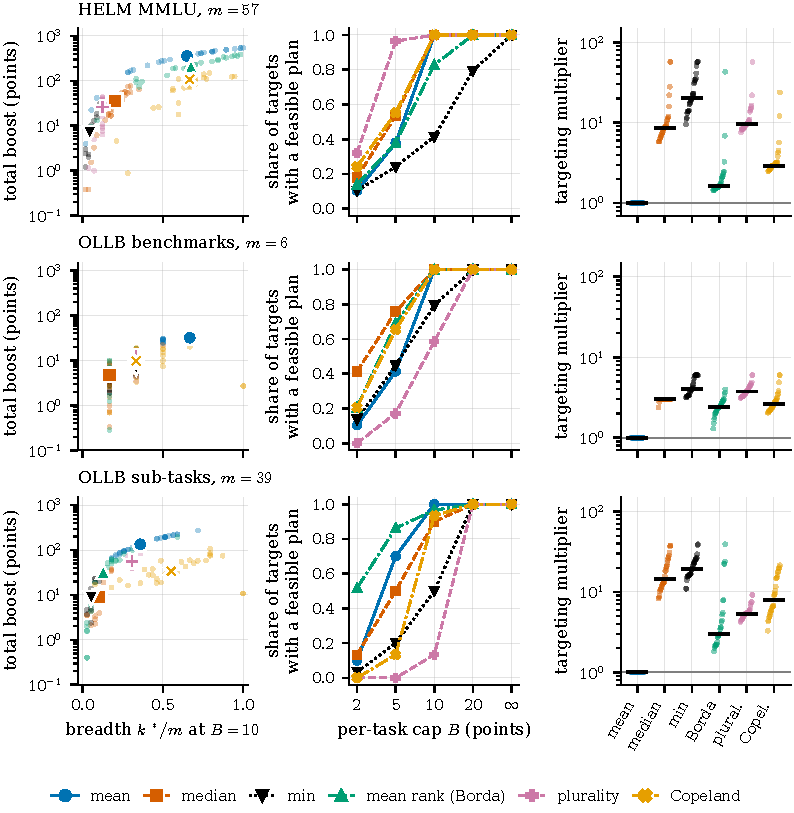
\includegraphics{../figures/fig2_price_map.pdf}
\caption{Price of first place for the 30 highest-ranked targets of each board (rows), against each rule's own leader; targets with zero gap are omitted. Left: total boost against breadth fraction at a per-task cap of 10 points (axes clipped at the bottom; one HELM and two benchmark-level targets within the tie margin of first place are off scale). Centre: share of targets with a feasible plan against the per-task cap. Right: targeting multiplier, the depth of the cheapest uniform plan over that of the cheapest targeted plan, at ceilings (two HELM and two sub-task targets off scale).}
\label{fig:map}
\end{figure}

\begin{figure}[h]
\centering
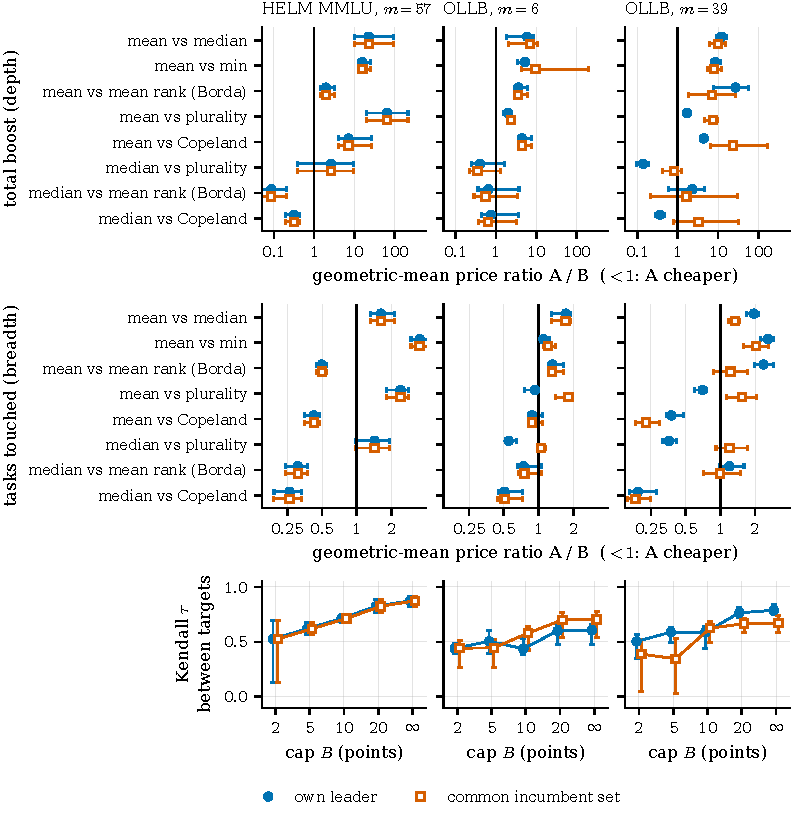
\includegraphics{../figures/fig4_pairs.pdf}
\caption{Paired price ratios between rules at a per-task cap of 20 points: geometric mean over targets of the price of the first rule divided by that of the second, with cluster-bootstrap 95\% intervals, for total boost (top) and for tasks touched (bottom), against each rule's own leader and a common incumbent set. Each cell uses 21--30 targets (targets already first under a rule are dropped). Ratios on the two sides of 1 show that no rule is cheapest throughout. The bottom row of panels shows the mean Kendall $\tau$ between the rule orderings of two targets against the per-task cap, with cluster-bootstrap 95\% intervals, again for own and common incumbents; it rises with the cap.}
\label{fig:paired}
\end{figure}

\begin{figure}[h]
\centering
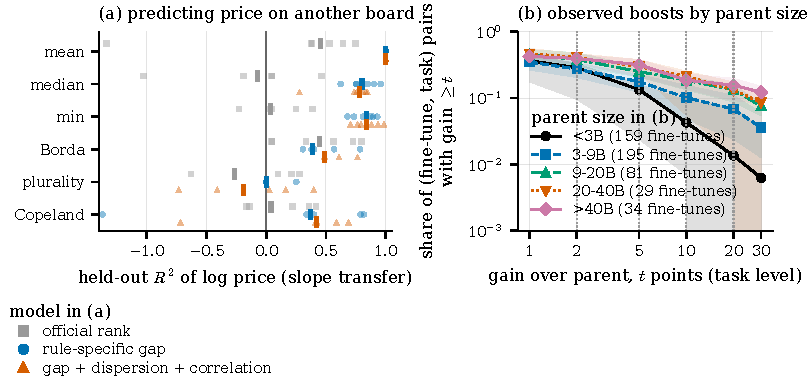
\includegraphics{../figures/fig5_predictors_calibration.pdf}
\caption{(a) Held-out $R^2$ of log price at ceilings when a model fitted on one board is applied to another with the slope transferred and the intercept re-estimated (the raw $R^2$ quoted for R3 is in \Cref{tab:verdicts}); 14 of 126 cells fall below $-1.4$ and are off the left edge. (b) Observed gains of fine-tuned models over their base models on the Open LLM Leaderboard: share of fine-tunes with a gain of at least a given number of points on some task, by parent size; grid lines at the budgets 2, 5, 10 and 20.}
\label{fig:calib}
\end{figure}

Detail of the calibration of \Cref{sec:calibration}. Open LLM Leaderboard models with a base model on the board give 159, 195, 81, 29 and 34 base--fine-tune pairs (from 21, 29, 13, 6 and 7 bases) for parents under 3B, 3--9B, 9--20B, 20--40B and over 40B. The median over children of the largest gain on any benchmark is 8, 9, 27, 34 and 36 points in these buckets, and the share of single-benchmark gains of at least 10 points rises from 4\% to 19--21\%. The budgets that matter (median minimal feasible budgets $B^\ast$ of 2 to 12 points, \Cref{tab:price}) lie within the range of the observed best-task gains only for parents of 9B and above: for 3--9B parents the median best-task gain is 9.3 (interval 5.7 to 20.0), below the larger budgets (11.5 for the minimum on HELM, 9.2 and 11.9 for plurality on the Open LLM Leaderboard). The top-30 targets are mostly models of 70B and above, for which the over-40B bucket has 34 children from 7 bases, and HELM's models have no observed pairs at all, so for them the scale is an assumption (\Cref{sec:discussion}); the pairs are not randomised, and a parent that is on the board is not always the model that was fine-tuned.

\section{Release and reproduction}
\label{app:release}

Every number in the paper is produced from the released analysis code and the result tables, which are anonymised for review. The inputs are the frozen public snapshots listed in \Cref{sec:data}: HELM MMLU release v1.13.0, and the Open LLM Leaderboard \texttt{contents} and \texttt{results} datasets at the commits given there. The code runs on CPU with Python 3.11, numpy 2.4, scipy 1.17, pandas 3.0 and HiGHS 1.16, and the random draws use fixed seeds. The exact price runs are the expensive part, about 77\,000 solver seconds in total on a shared CPU host (a few seconds to a half minute per target and rule on the largest boards, with a 30\,s limit per integer program); the figure is an upper bound on CPU time because the host was loaded. The licences of the data are those of their sources, and only processed numbers are redistributed.
